\documentclass[11pt]{beamer}
\usetheme{Madrid}
\usefonttheme{serif}

\usepackage[utf8]{inputenc}
\usepackage[spanish]{babel}
\usepackage[T1]{fontenc}

\usepackage{amsmath}
\usepackage{amsfonts}
\usepackage{amssymb}
\usepackage{graphicx, xcolor}
\usepackage{listings}
\usepackage{array}
\usepackage{colortbl}
\usepackage{xcolor}

\usepackage[absolute,overlay]{textpos}
\usepackage[most]{tcolorbox}

\usepackage{url}
\usepackage{natbib}
\usepackage{ragged2e}
\usepackage{lipsum,framed}

\usepackage{tikz}
\usetikzlibrary{shapes.geometric, arrows.meta, positioning, calc, automata}
\usetikzlibrary{shapes, arrows}

\tikzstyle{startstop} = [rectangle, rounded corners, minimum width=3cm, minimum height=1cm,text centered, draw=black, fill=red!30]
\tikzstyle{process} = [rectangle, minimum width=3cm, minimum height=1cm, text centered, draw=black, fill=blue!20]
\tikzstyle{decision} = [diamond, aspect=2, minimum width=3.5cm, minimum height=1cm, text centered, draw=black, fill=yellow!40]
\tikzstyle{arrow} = [thick, ->, >=Stealth]

\tikzset{
block/.style={rectangle, draw, fill=gray!30, text centered, rounded corners, minimum height=1cm, minimum width=3cm},
ovalblock/.style={ellipse, draw, fill=gray!30, text centered, minimum height=1cm, minimum width=3cm},
line/.style={-Stealth, thick},
}


%\tikzstyle{cloud} = [draw, ellipse,fill=gray!40,
%minimum height=2em, minimum width=4em]
%\tikzstyle{block} = [draw, rectangle, minimum height=1cm, minimum width=0.5cm, fill=gray!20]
%\tikzstyle{module} = [draw, rectangle, minimum height=4cm, minimum width=6cm]
%\tikzstyle{line} = [draw, -latex']


\DeclareMathOperator{\sen}{sen}
\DeclareMathOperator{\tg}{tg}

\setbeamertemplate{caption}[numbered]

%\setbeameroption{show notes on second screen=right}  % También puedes usar: show notes on second screen=right

\author[LLO]{Ing. Leonardo Luis Ortiz}
\title{Introducción a la programación RTL en C++ para simulación de procesamientos digitales de señales}
% Informe su email de contato o comando a seguir
% Por ejemplo, alcebiades.col@ufes.br
\newcommand{\email}{leonardo.ortiz@ib.edu.ar}
%\setbeamercovered{transparent} 
\setbeamertemplate{navigation symbols}{} 
\logo{\includegraphics[scale=0.08]{images/IB.png}} 
\institute[]{Instituto Balseiro \par Centro Atómico Bariloche} 
\date{\today} 
%\subject{}

% ---------------------------------------------------------
% Selecione un estilo de referencia
\bibliographystyle{apalike}

%\bibliographystyle{abbrv}
%\setbeamertemplate{bibliography item}{\insertbiblabel}
% ---------------------------------------------------------

% ---------------------------------------------------------
% Incluir los slides 
%\usepackage[spanish,hyperpageref]{backref}

%\renewcommand{\backrefpagesname}{Cita de página(s):~}
%\renewcommand{\backref}{}
%\renewcommand*{\backrefalt}[4]{
	%	\ifcase #1 %
	%		Sin citas en el texto.%
	%	\or
	%		Citado en la página #2.%
	%	\else
	%		Citado #1 veces en las páginas #2.%
	%	\fi}%
% ---------------------------------------------------------
%% Configuración para el código
%\lstset{
%	language=C++,
%	basicstyle=\ttfamily\scriptsize,
%	keywordstyle=\color{blue},
%	commentstyle=\color{gray},
%	stringstyle=\color{orange},
%	showstringspaces=false,
%	breaklines=true,
%	frame=single,
%	numbers=left,
%	numberstyle=\tiny,
%	tabsize=2
%}

% Estilo para VHDL
\lstdefinelanguage{VHDL}{
	morekeywords={
		library,use,all,entity,is,port,in,out,end,architecture,of,begin,
		signal,process,if,then,else,elsif,wait,until,when,others
	},
	sensitive=true,
	morecomment=[l]--,
	morestring=[b]"
}

\lstset{
	language=VHDL,
	basicstyle=\ttfamily\scriptsize,
	keywordstyle=\color{blue},
	commentstyle=\color{gray},
	stringstyle=\color{orange},
	showstringspaces=false,
	breaklines=true,
	frame=single,
	numbers=left,
	numberstyle=\tiny,
	tabsize=2,
	captionpos=b
}


\begin{document}
	
	\begin{frame}
		\titlepage
	\end{frame}
	
	\begin{frame}{Objetivos}
	\begin{itemize}
		\item El dictado del curso se orienta a proveer al alumno de la capacidad de diseñar sistemas de procesamiento de señal, y utilizar el simulador HALCON como herramienta para la verificación y análisis.
	\end{itemize}
	\end{frame}
	
	\begin{frame}{Contenido}
		\tableofcontents 
	\end{frame}
	
%	\begin{frame}{Event-Driven Programming}
%	Contenidos:	\newline
%	\begin{itemize}
%		\item Introducción
%		\item Componentes de un Sistema controlado por Eventos
%		\item Flujo de Eventos y Gestión de Eventos
%		\item Arquitectura Controlada por Eventos (EDA)
%		\item Fuentes de Eventos y Tipos de Eventos
%		\item Modelos de Concurrencia Controlada por Eventos
%	\end{itemize}
%	\end{frame}
	
	\section{Introducción}
	\begin{frame}{Event-Driven Programming}
	\huge \centering
	\textbf{Introducción}
	\end{frame}
	
	\begin{frame}{Introducción}
		\small
	La Programación controlada por Eventos (Event-driven Programming - EDP) es un paradigma donde el flujo de un programa está determinado por eventos, en lugar de una secuencia predefinida de instrucciones. Los eventos pueden activarse mediante interacciones del usuario, señales del sistema o fuentes externas. \newline
	\textbf{“Un evento es un hecho inmutable, algo que ha sucedido en el pasado y que no se puede cambiar”.}
	
	\begin{center}
	\begin{tikzpicture}[
		node distance=1.0cm and 1.8cm,
		every node/.style={font=\small},
		box/.style={draw=green!40!black, minimum width=2.8cm, minimum height=1cm, align=center},
		arrow/.style={thick, ->, >=Stealth, draw=green!50!black}
		]
		
		% Nodos
		\node[box] (dispatcher) {dispatcher};
		\node[box, below left=of dispatcher] (handler1) {handler 1};
		\node[box, below=of dispatcher] (handler2) {handler 2};
		\node[box, below right=of dispatcher] (handlern) {handler n};
		
		% Texto "events"
		\node[above=0.4cm of dispatcher] (events) {\textcolor{green!50!black}{\textbf{events}}};
		
		% Flechas
		\draw[->, thick] (events) -- (dispatcher);
		\draw[->, thick] (dispatcher.south west) -- (handler1.north);
		\draw[->, thick] (dispatcher.south) -- (handler2.north);
		\draw[->, thick] (dispatcher.south east) -- (handlern.north);
		
		% Puntos suspensivos
		\node[xshift=3cm, yshift=-2.5cm] at ($(handler2)!0.5!(handlern)$) {\Large $\cdots$};
		
		% Texto debajo
		\node[below=3.2cm of dispatcher] {\textbf{\textcolor{blue!50!black}{\textsc{Handlers pattern}}}};
	\end{tikzpicture}
	\end{center}
	
		
	\end{frame}
	
	\begin{frame}{Event-Driven Programming}
%		Componentes de EDP:
%		\begin{itemize}
%			\item Event listeners: detectan los eventos
%			\item Events handlers: ejecutan la respuesta a eventos
%			\item Event loops: monitorean continuamente nuevos eventos
%		\end{itemize} 
%		\vspace{1cm}

		Ciclo de vida de EDP:
		\begin{itemize}
			\item \textbf{Generación de eventos}: Los eventos pueden generarse mediante la entrada del usuario, procesos en segundo plano, señales de hardware o comunicaciones externas. Algunos ejemplos incluyen hacer clic en un botón, recibir una solicitud HTTP o detectar movimiento de un sensor.
			\item \textbf{Detección de eventos}: Un detector de eventos monitoriza eventos específicos y notifica al sistema cuando ocurren. Este mecanismo garantiza una respuesta en tiempo real.
			\item \textbf{Gestión de eventos}: Una vez detectado un evento, el controlador correspondiente ejecuta una función predefinida para procesarlo. Esto puede implicar actualizar una interfaz de usuario, procesar datos o enviar solicitudes de red.
			
		\end{itemize}	
			
	\end{frame}
	
	\begin{frame}{Event-Driven Programming - Características}
	\begin{itemize}
		\item \textbf{Ejecución asíncrona}: a diferencia de la programación secuencial tradicional, la EDP permite que los controladores de eventos se ejecuten de forma independiente sin bloquear otras operaciones.
		\item \textbf{Desacoplamiento de componentes}: los eventos facilitan el diseño modular, lo que permite que las diferentes partes de una aplicación interactúen sin dependencias directas.
		\item \textbf{Funciones de callbacks}: los handlers de eventos suelen implementarse como callbacks, que se invocan cuando ocurre un evento específico.
		\item \textbf{Lógica basada en el estado (State-Driven Logic)}: el comportamiento de la aplicación se determina por la ocurrencia de eventos, en lugar de un flujo de control fijo.
	\end{itemize} 
	\end{frame}
	
	\begin{frame}{Event-Driven Programming - Ventajas}
		\small
	\begin{itemize}
		\item \textbf{Ejecución Asincrónica}: A diferencia de la ejecución secuencial, los sistemas basados en eventos pueden gestionar múltiples tareas simultáneamente, lo que mejora la capacidad de respuesta. Esto es fundamental en aplicaciones como servidores web, donde varios usuarios interactúan simultáneamente.
		\item \textbf{Escalabilidad mejorada}: EDP permite gestionar eventos de gran volumen de forma eficiente, lo que la hace ideal para microservicios, arquitecturas sin servidor y aplicaciones en tiempo real.
		\item \textbf{Diseño modular y extensible}: Los eventos desacoplan los componentes, lo que permite un código flexible y reutilizable. Los desarrolladores pueden modificar los controladores de eventos de forma independiente sin afectar a todo el sistema.
		\item \textbf{Tiempo de inactividad de la CPU reducido}: Dado que los loops de eventos monitorizan y distribuyen eventos continuamente, los recursos de la CPU se utilizan eficazmente, lo que hace que EDP sea ideal para aplicaciones de baja latencia.
	\end{itemize} 
	\end{frame}

	\begin{frame}{Event-Driven Programming - Desafíos}
	\small
	\begin{itemize}
	\item \textbf{Difícil depuración y testeo}: La ejecución asíncrona dificulta el seguimiento de secuencias de eventos y la reproducción de problemas. Las herramientas de depuración, como los registros de eventos (event logs) y los frameworks de seguimiento, son esenciales.
	\item \textbf{Problemas con las callbacks}: Anidar múltiples devoluciones de llamadas puede generar código espagueti, lo que reduce la legibilidad y el mantenimiento. Las promesas y los patrones async/await mitigan este problema.
	\item \textbf{Complejidad en la Gestión del Estado}: Gestionar múltiples eventos simultáneos requiere una sincronización cuidadosa para evitar condiciones de carrera e inconsistencias en los datos.
	\item \textbf{Consumo de Memoria}: Los escuchas de eventos de larga duración pueden consumir memoria con el tiempo, lo que puede provocar fugas de memoria si no se gestionan adecuadamente.
	\end{itemize} 
	\end{frame}


	\begin{frame}{Event-Driven Programming - Aplicaciones}
	\begin{itemize}
		\item \textbf{GUI applications (Graphical User Interface)}
		\item \textbf{Cloud-base microservices}
		\item \textbf{IoT devices} 
		\item \textbf{Real Time Systems (RTS)}
		\item \textbf{Networking}
		\item \textbf{Distribuided Systems}
	\end{itemize} 
	\end{frame}

	% ************************************************************
	% Module 2
	% ***********************************************************
	\section{Componentes de un Sistema Basado en Eventos}
	
	\begin{frame}{Event-Driven Programming}
		\huge \centering
		\textbf{Componentes de un Sistema Basado en Eventos}
	\end{frame}

	\begin{frame}[fragile]{Event-Driven Programming}
	\small 
	Un sistema basado en eventos consta de múltiples componentes que trabajan en conjunto para garantizar un procesamiento eficiente de eventos. Los elementos clave incluyen \textbf{productores de eventos} y \textbf{consumidores de eventos}, que generan y procesan eventos; \textbf{event loops} y \textbf{event handlers}, que gestionan la ejecución asíncrona; \textbf{event listeners} y \textbf{dispatchers}, que detectan y distribuyen loseventos; y \textbf{middleware}, que facilita la comunicación y el flujo de eventos. 
	\begin{center}
	\begin{tikzpicture}[
	node distance=1.0cm and 1.8cm,
	every node/.style={font=\small},
	box/.style={draw=green!40!black, minimum width=2.8cm, minimum height=1cm, align=center},
	arrow/.style={thick, ->, >=Stealth, draw=green!50!black}
	]
	
	% Nodos
	\node[box] (dispatcher) {dispatcher};
	\node[box, below left=of dispatcher] (handler1) {handler 1};
	\node[box, below=of dispatcher] (handler2) {handler 2};
	\node[box, below right=of dispatcher] (handlern) {handler n};
	
	% Texto "events"
	\node[above=0.4cm of dispatcher] (events) {\textcolor{green!50!black}{\textbf{events}}};
	
	% Flechas
	\draw[->, thick] (events) -- (dispatcher);
	\draw[->, thick] (dispatcher.south west) -- (handler1.north);
	\draw[->, thick] (dispatcher.south) -- (handler2.north);
	\draw[->, thick] (dispatcher.south east) -- (handlern.north);
	
	% Puntos suspensivos
	\node[xshift=3cm, yshift=-2.5cm] at ($(handler2)!0.5!(handlern)$) {\Large $\cdots$};
	
	% Texto debajo
	\node[below=3.2cm of dispatcher] {\textbf{\textcolor{blue!50!black}{\textsc{Handlers pattern}}}};
	\end{tikzpicture}
	\end{center}
	\end{frame}
	
	\begin{frame}{Modelo Event Producers \& Consumers}
		\small \justifying
		En una arquitectura basada en eventos, los \textbf{productores de eventos} generan eventos, mientras que los \textbf{consumidores} los procesan. Los productores pueden incluir interacciones del usuario (clics del ratón, pulsaciones de teclas), eventos del sistema (actualizaciones de archivos, solicitudes de red) o fuentes externas (llamadas a API, sensores IoT). Los consumidores son responsables de gestionar estos eventos y ejecutar las acciones pertinentes. \\
		Los productores y consumidores de eventos operan de forma \textbf{independiente}, lo que hace que los sistemas basados en eventos sean altamente escalables y estén débilmente acoplados. Esta disociación permite a los productores enviar eventos sin saber cómo ni cuándo los procesarán los consumidores. Para optimizar la comunicación, los sistemas suelen utilizar colas de mensajes (\textbf{event queues}) o \textbf{event brokers} para gestionar el flujo de eventos. Entre los ejemplos de productores de eventos se incluyen las interfaces de usuario, los servidores web y los sistemas de monitorización en tiempo real, mientras que los consumidores pueden ser servicios de registro, gestores de notificaciones o tareas en segundo plano.
	\end{frame}

	\begin{frame}[fragile]{Modelo Event Producers \& Consumers}
		\small
	\begin{center}	
	\begin{tikzpicture}[
		node distance=0.5cm and 0.8cm,
		every node/.style={font=\small},
		box/.style={draw=green!40!black, minimum width=2.8cm, minimum height=1cm, align=center},
		arrow/.style={thick, ->, >=Stealth, draw=green!50!black}
		]
		
		% Nodos
		\node[box] (producers) {{\bfseries Producers} \\(user interfaces, \\system processes,\\ IoT sensors, APIs)};
		\node[box, right=of producers] (queue) {{\bfseries Message queue} \\ {\bfseries Event brokers}};
		\node[box, right=of queue] (consumers) {{\bfseries Consumers} \\ (logging, \\ data updates, \\triggering other\\ processes)};
		
		% Flechas
		\draw[->, thick] (producers) -- (queue);
		\draw[->, thick] (queue) -- (consumers);
		
	\end{tikzpicture}
	\end{center}
	\end{frame}
	
	\begin{frame}{Modelo Event Producers \& Consumers: Producers}
	\small
	Los productores de eventos inician el flujo de eventos emitiendo señales para notificar cambios al sistema. Se pueden clasificar en:
	
	\begin{itemize}
	\item \textbf{Producers generados por el usuario} : aplicaciones GUI donde los usuarios interactúan mediante botones, pulsaciones de teclas o gestos.
	\item \textbf{Producers generados por el sistema} : aplicaciones GUI donde los usuarios interactúan mediante botones, pulsaciones de teclas o gestos.
	\item \textbf{Producers externos} : webhooks, API, dispositivos IoT o servicios en la nube que activan flujos de trabajo basados en eventos.
	\end{itemize} 
	\vspace{1cm}
	Los \textbf{Producers} no suelen esperar la respuesta de los \textbf{Consumers}. En su lugar, publican eventos en un \textbf{bus de eventos}, \textbf{cola de mensajes} o un \textbf{broker}, lo que garantiza la escalabilidad y la ejecución asincrónica.

	\end{frame}

	\begin{frame}{Modelo Event Producers \& Consumers: Producers}
	\small
	\begin{itemize}
		\item \textbf{Consumer único} : Un consumidor procesa un tipo de evento específico (p. ej., un observador de archivos que actualiza una base de datos).
		\item \textbf{Múltiples consumers} : Varios controladores procesan el mismo evento (p. ej., una notificación por correo electrónico y un sistema de registro que responden a un evento de registro de usuario).
		\item \textbf{Event pipelines} :Los eventos disparan procesos secuenciales (p. ej., un sensor de IoT que envía datos → se almacenan en una base de datos → se analizan en tiempo real).
	\end{itemize} 
	\vspace{1cm}
	Los consumers utilizan controladores basados en eventos para ejecutar tareas al recibir un evento, lo que permite que el sistema responda a los cambios en tiempo real.
	\end{frame}
	
	
	\begin{frame}{Event loops \& Handlers}
	\small \justifying
	Los loops y handlers (controladores) de eventos son componentes esenciales de la programación basada en eventos, lo que permite la ejecución asíncrona y un procesamiento eficiente de eventos. El loop de eventos es un ciclo continuo que detecta los eventos entrantes y los envía a controladores registrados para su ejecución. Los handlers de eventos son funciones o callbacks que procesan eventos específicos, garantizando la capacidad de respuesta de la aplicación. Estos componentes son esenciales en interfaces gráficas de usuario (GUI), servidores web, aplicaciones de red y sistemas en tiempo real.
	\end{frame}

	\begin{frame}{Event loops \& Handlers: Event Loop}
	\small
	\begin{itemize}
		\item \textbf{Event Detection}: Monitorea los eventos entrantes desde colas, sockets o listeners.
		\item \textbf{Event Dispatching}: Asigna los eventos detectados a los handlers correspondientes.
		\item \textbf{Event Execution}: Procesa el evento mediante el handler correspondiente.
		\item \textbf{Idle State}: Espera nuevos eventos cuando no hay ninguno pendiente.
	\end{itemize} 
	\vspace{1cm}
	Al gestionar múltiples eventos de forma asincrónica, los bucles de eventos evitan que las aplicaciones se bloqueen en tareas individuales, lo que mejora significativamente la eficiencia y la escalabilidad.
	\end{frame}
	
	\begin{frame}{Event loops \& Handlers: Event Handlers}
	\small
	Un controlador de eventos es una función que se ejecuta cuando ocurre un evento específico. Los controladores deben ser no bloqueantes para evitar cuellos de botella en el rendimiento del loop de eventos. Pueden ser:
	\begin{itemize}
		\item \textbf{Controladores síncronos}: se ejecutan secuencialmente, esperando a que se complete la ejecución antes de procesar el siguiente evento.
		\item \textbf{Controladores asíncronos}: utilizan operaciones no bloqueantes (por ejemplo, async/await en Python) para gestionar varios eventos simultáneamente.
	\end{itemize} 
	\vspace{1cm}
	Un manejo eficiente de eventos evita \textbf{race conditions}, \textbf{callback hell} y \textbf{degradación del rendimiento}.
	\end{frame}

	\begin{frame}{Event Listeners \& Dispatchers}
	\justifying
	Los \textbf{listeners} y \textbf{dispatchers} de eventos son fundamentales para las arquitecturas basadas en eventos, ya que permiten la detección y distribución eficiente de eventos. Un \textbf{listener} de eventos monitoriza eventos específicos y reacciona cuando ocurren, mientras que un \textbf{dispatcher} de eventos garantiza que el evento se enrute al controlador correcto. Estos componentes permiten que las aplicaciones sean responsivas, modulares y escalables al desvincular a los producers de eventos de los consumers.
	\end{frame}
	
	\begin{frame}{Event Listeners \& Dispatchers: Listeners}
	\small
	Algunos casos de uso comunes incluyen:
	\begin{itemize}
		\item \textbf{Aplicaciones GUI}: Los listeners detectan clics de botones, movimientos del ratón y pulsado de teclas.
		\item \textbf{Aplicaciones web}: monitorizan solicitudes HTTP, conexiones WebSocket y actualizaciones en la base de datos.
		\item \textbf{Sistemas IoT}: Los dispositivos ``escuchan'' actualizaciones de datos de sensores o señales externas.
	\end{itemize} 
	\vspace{1cm}
	Los Listeners registran eventos específicos y ejecutan las callbacks asignadas cuando ocurren. Pueden ser síncronos o asíncronos, según los requisitos del sistema.
	\end{frame}
	
	\begin{frame}{Event Listeners \& Dispatchers: Dispatchers}
	\small
	Un dispatcher de eventos dirige los eventos detectados a los controladores adecuados. Garantiza que los eventos lleguen a los componentes correctos, lo que permite un procesamiento modular de eventos. \\
	\vspace{0.5cm}
	Los despachadores pueden operar en diferentes modos:
	\vspace{0.3cm}
	\begin{itemize}
		\item \textbf{Direct Dispatching}: los eventos se envían directamente a un único controlador predefinido.
		\item \textbf{Broadcasting}: los eventos se envían a múltiples suscriptores (modelo publish-subscribe).
		\item \textbf{Queue-Based Dispatching}: los eventos se ponen en cola y se procesan en orden.
	\end{itemize} 
	\vspace{0.5cm}
	Un despacho eficiente optimiza el rendimiento al garantizar que los eventos no bloqueen la ejecución mientras esperan su procesamiento.

	\end{frame}

	\begin{frame}{Event Listeners \& Dispatchers: Dispatchers}
	\begin{figure}[htb]
		\centering
		\includegraphics[width=1\textwidth]{images/Event_queue}
	\end{figure}
	\end{frame}
	
	\begin{frame}{Middleware}
	\small \justifying
	El \textbf{middleware} en sistemas basados en eventos actúa como una capa intermedia que facilita la comunicación, el procesamiento de eventos y el enrutamiento de mensajes entre los producers y los consumers de eventos. Proporciona servicios esenciales como el filtrado de eventos, transformaciones, logging, seguridad y la gestión de colas de mensajes, garantizando la escalabilidad, la fiabilidad y el desacoplamiento en arquitecturas distribuidas. El middleware se utiliza ampliamente en microservicios, aplicaciones en tiempo real y sistemas empresariales basados en eventos para gestionar eficientemente flujos de eventos complejos.\newline
	
	\begin{itemize}
		\item RabbitMQ
		\item Apache Kafka
		\item Redis Pub/Sub
	\end{itemize}
	\end{frame}
	
	\begin{frame}{Middleware}
	\small
	El middleware mejora los sistemas basados eneventos gestionando el pre-procesamiento y el pos-procesamiento de eventos. Algunas de sus responsabilidades clave son:
	\begin{itemize}
	\item \textbf{Filtrado de eventos}: Selecciona eventos relevantes según reglas predefinidas, evitando el procesamiento innecesario.
	\item \textbf{Transformación de eventos}: Convierte formatos de eventos para garantizar la compatibilidad entre servicios (p. ej., JSON a XML).
	\item \textbf{Enrutamiento de mensajes}: Dirige los eventos a los consumers adecuados en arquitecturas de publicación-suscripción.
	\item \textbf{Seguridad y autenticación}: Garantiza la transmisión segura de eventos entre componentes.
	item \textbf{Logging y monitoreo}: Rastrea los flujos de eventos para su depuración y análisis.
	\end{itemize} 
	\vspace{0.3cm}
	El middleware garantiza el correcto funcionamiento de las arquitecturas basadas en eventos en entornos distribuidos, estandarizando la transmisión de eventos y reduciendo la complejidad del sistema.
	\end{frame}
	
	% ************************************************************
	% Module 3
	% ***********************************************************
	\section{Flujo de Eventos y Gestión de Eventos}

	\begin{frame}{Event-Driven Programming}
		\huge \centering
		\textbf{Flujo de Eventos \\y \\Gestión de Eventos}
	\end{frame}
	
	\begin{frame}{Event Flow \& Event Handling}
	\justifying
	El flujo y la gestión de eventos definen cómo se propagan los eventos a través de una aplicación y cómo se procesan. Un flujo de eventos estructurado garantiza una gestión de eventos eficiente y organizada, evitando conflictos y operaciones redundantes. Comprender la propagación de eventos, los mecanismos de gestión y la secuenciación es crucial para diseñar sistemas basados en eventos escalables y con capacidad de respuesta en aplicaciones GUI, desarrollo web y computación distribuida.
	
	\end{frame}

	\begin{frame}{Propagación de eventos}
	\small
	La propagación de eventos determina cómo se mueven los eventos a través de la jerarquía de componentes de una aplicación. En interfaces gráficas de usuario (GUI), aplicaciones web y sistemas basados en mensajes, los eventos viajan a través de múltiples elementos antes de ser procesados. La propagación sigue una secuencia estructurada, lo que garantiza que los oyentes de eventos en diferentes niveles puedan responder adecuadamente. \\Los dos modelos de propagación principales son:
	\begin{itemize}
		\item \textbf{De arriba a abajo (fase de captura)}: Los eventos viajan desde el elemento raíz hasta el elemento de destino.
		\item \textbf{De abajo a arriba (fase de propagación)}: Los eventos se originan en el elemento de destino y se propagan hacia arriba.
	\end{itemize}
	Controlar la propagación de eventos ayuda a los desarrolladores a gestionar conflictos de eventos, optimizar el rendimiento e implementar comportamientos complejos basados en eventos, como la delegación y la interceptación.
	\end{frame}

	\begin{frame}{Control de Eventos: Síncronos \& Asíncronos}
		\small
	Los sistemas basados en eventos pueden gestionar eventos de forma síncrona o asíncrona, según los requisitos de rendimiento y capacidad de respuesta.
	\begin{itemize}
		\item \textbf{Synchronous Handling}: Los eventos se procesan secuencialmente, bloqueando la ejecución hasta que el handler finaliza. Esto garantiza un orden predecible, pero puede causar retrasos en aplicaciones con alto tráfico.
		\item \textbf{Asynchronous Handling}: Los eventos se ejecutan simultáneamente, lo que evita bloqueos y mejora la capacidad de respuesta. Esto es fundamental para las operaciones de red, las aplicaciones en tiempo real y los sistemas basados en eventos a gran escala.
	\end{itemize}
	La elección entre modelos síncronos y asíncronos depende de factores como las dependencias de los eventos, el tiempo de ejecución y las necesidades de concurrencia.
	Una gestión eficiente de eventos mejora la experiencia del usuario y el rendimiento de las aplicaciones.	
	\end{frame}
	
	
	\begin{frame}{Control de Eventos: Síncronos \& Asíncronos}
		\small
		\begin{table}
			\centering
			\renewcommand{\arraystretch}{1.2}
			\begin{tabular}{|p{3cm}|p{4cm}|p{4cm}|}
				\hline
				\textbf{Característica} & \textbf{Síncrono} & \textbf{Asíncrono} \\ \hline
				\textbf{Orden de ejecución} & Secuencial & Concurrente \\ \hline
				\textbf{Conducta} & Bloqueante & No bloqueante \\ \hline
				\textbf{Performance} & Lento & Rápido \\ \hline
				\textbf{Complejidad} & Fácil & Más complejo \\ \hline
				\textbf{Casos de uso} & 
				Tareas simples, aplicaciones de baja latencia &
				Aplicaciones de alta performance, operaciones pesadas de E/S \\ \hline
			\end{tabular}
		\end{table}
	\end{frame}
	
	
	\begin{frame}{Gestión de Secuencias de Eventos y Dependencias}
	\small
	En aplicaciones complejas basadas en eventos, varios eventos ocurren en secuencia, a veces con dependencias entre ellos. Gestionar las secuencias de eventos garantiza un orden de ejecución correcto y evita conflictos. \\
	Las estrategias clave para gestionar las dependencias de eventos incluyen:	
	
	\begin{itemize}
		\item \textbf{Event Queues}: organizan eventos en una secuencia estructurada para evitar conflictos.
		\item \textbf{Callbacks \& Promises}: garantizan que los eventos dependientes se ejecuten en el orden correcto.
		\item \textbf{Event Prioritization}: asignan niveles de prioridad a eventos críticos.
	\end{itemize}
	Una secuencia de eventos bien gestionada previene condiciones de carrera, deadlocks (bloqueos) y comportamientos imprevistos, lo que garantiza un rendimiento fluido de la aplicación.
	El flujo y la gestión de eventos definen cómo responden las aplicaciones a las acciones del usuario y a los eventos del sistema. Un control de propagación adecuado, estrategias de gestión y gestión de dependencias permiten a los desarrolladores crear arquitecturas basadas en eventos eficientes, ágiles y fáciles de mantener. 
	\end{frame}
	
	\begin{frame}{Secuenciación de eventos}
		La secuenciación de eventos define el orden en que se ejecutan para mantener un flujo lógico. Algunos eventos pueden necesitar ejecutarse antes que otros debido a dependencias de datos, reglas de negocio o restricciones del sistema.\\
	Estrategias para la secuenciación de eventos:
	\begin{itemize}
		\item \textbf{Ordenación manual}: Defina reglas explícitas para ejecutar eventos en una secuencia fija.
	\item \textbf{Ejecución basada en prioridad}: Asignar niveles de prioridad a los eventos para garantizar que las tareas de mayor prioridad se ejecuten primero.
	\item \textbf{Ejecución basada en estado}: Ejecutar eventos solo cuando un sistema alcanza un estado específico (por ejemplo, esperar la entrada del usuario antes de enviar un formulario).
	\end{itemize}	
	\end{frame}
	
	\begin{frame}{Dependencias de eventos}
	Algunos eventos no pueden ejecutarse hasta que se completen los eventos prerequisito. Las dependencias deben gestionarse con cuidado para evitar interbloqueos, condiciones de carrera y transiciones de estado inconsistentes.\newline
	\\
	Tipos de dependencias de eventos:
	\begin{itemize}
		\item \textbf{Dependencias rígidas}: Un evento debe completarse antes de que comience otro. Ejemplo: Una actualización de la base de datos debe finalizar antes de enviar un correo electrónico de confirmación.
	\item \textbf{Dependencias blandas}: Algunos eventos pueden ejecutarse en paralelo, pero puede ser necesaria la sincronización. Ejemplo: Varios microservicios procesan solicitudes de usuario simultáneamente.	
	\end{itemize}
	\end{frame}
	
	
	% **************************************************************
	%                   Module 5 
	% **************************************************************
	\section{Arquitectura Basada en Eventos (EDA)}
	
	\begin{frame}{Event-Driven Programming}
		\huge \centering
		\textbf{Arquitectura Basada en Eventos (EDA)}
	\end{frame}
	
	\begin{frame}{Event-Driven Architecture (EDA)}
	\small
	La Arquitectura Basada en Eventos (EDA) es un paradigma de diseño de software donde los componentes del sistema interactúan principalmente mediante la generación, detección y respuesta a eventos. A diferencia de los modelos tradicionales de solicitud-respuesta, la EDA permite la comunicación asíncrona, alta escalabilidad y flexibilidad, lo que la hace ideal para aplicaciones en tiempo real, microservicios y sistemas distribuidos.
	
	\textbf{Principios de la Arquitectura Basada en Eventos}\\
	La EDA se basa en un enfoque descentralizado y reactivo, donde los sistemas responden dinámicamente a los eventos en lugar de seguir un flujo de trabajo rígido. \\
	
	\begin{itemize}
		\item \textbf{Event Producers \& Consumers}: Componentes que generan y responden a eventos de forma independiente.
		\item \textbf{Brokers de Eventos y Middleware}: Facilitan la transmisión de eventos entre componentes desacoplados.
		\item \textbf{Procesamiento Asíncrono}: Los eventos se gestionan sin bloquear otros procesos, lo que mejora la eficiencia. 
		\item \textbf{Escalabilidad y tolerancia a fallos}: la gestión independiente de eventos permite el escalamiento horizontal y la resiliencia.
	\end{itemize}
	\end{frame}
	
	\begin{frame}{Event-Driven Architecture (EDA)}
		\begin{table}
		\centering
		\renewcommand{\arraystretch}{1.2}
		\begin{tabular}{|p{3cm}|p{4cm}|p{4cm}|}
			\hline
			\textbf{Característica} & \textbf{Arquitectura Tradicional} & \textbf{Arquitectura Basada en Eventos} \\ \hline
			\textbf{Comunicación} & Directa, Sincrónica & Indirecta, Asincrónica \\ \hline
			\textbf{Escalabilidad} & Limitada & Altamente escalable \\ \hline
			\textbf{Flexibilidad} & Fuertemente acoplado & Débilmente acoplado \\ \hline
			\textbf{Perfomance} & Ejecución bloqueante & Ejecución no bloqueante \\ \hline
			\textbf{Control de errores} & Reintentos síncrónicos & Reintentos asincrónicos con registros de eventos \\ \hline
			\end{tabular}
		\end{table}
	\end{frame}
	
	\begin{frame}{Estrategias para la escalabilidad en EDA}
	
	\begin{itemize}
		\item \textbf{Procesamiento asíncrono de eventos}: Uso de colas de mensajes (p. ej., RabbitMQ, Kafka) para procesar eventos en paralelo sin bloquear la ejecución.
		\item \textbf{Balanceo de carga}: Distribución del procesamiento de eventos entre múltiples consumidores para evitar la sobrecarga.
		\item \textbf{Particionamiento de eventos}: División de flujos de eventos en particiones más pequeñas para su consumo en paralelo.
		\item \textbf{Agregado y filtrado de eventos}: Reducción del procesamiento redundante mediante la agrupación de eventos o el filtrado de los innecesarios antes de su procesamiento.
		\item \textbf{Escalado automático}: Ajuste dinámico de recursos (p. ej., AWS Lambda, Kubernetes) en función de la carga de eventos.
	\end{itemize}
	\end{frame}
	
	\begin{frame}{Fuentes y Tipos de Eventos}
		\huge \centering
		\textbf{Fuentes y Tipos de Eventos}
	\end{frame}
	
	\begin{frame}{Fuentes y Tipos de Eventos}
	\begin{itemize}
		\item \textbf{Eventos de Interface Usuario (UI)}
		\item \textbf{Eventos del Sistema y Hardware}
		\item \textbf{Eventos de Red y E/S}
		\item \textbf{Eventos personalizados} (específicos de la aplicación)
	\end{itemize}	
	\end{frame}
	
	\begin{frame}{Eventos de Interface Usuario (UI)}
		\begin{itemize}
			\item \textbf{Eventos del mouse}: clic, doble clic, pulsar el ratón, subir el ratón, mover el ratón, pasar el ratón por encima, salir del ratón.
			\item \textbf{Eventos del teclado}: pulsar tecla, tecla subir, tecla subir.
			\item \textbf{Eventos táctiles}: iniciar, mover, finalizar.
			\item \textbf{Eventos de Formulario}: introducir, cambiar, enviar, restablecer.
			\item \textbf{Eventos de Ventana}: redimensionar, desplazar, enfocar, desenfocar.
		\end{itemize}	
	\end{frame}
	
	\begin{frame}{Eventos del Sistema y Hardware}
		\begin{itemize}
			\item \textbf{Eventos de Energía}: Inicio, apagado, suspensión o cambios en el estado de la batería del sistema.
			\item \textbf{Eventos del dispositivo}: Conexiones USB, detección de hardware externo o extracción de dispositivos.
			\item \textbf{Eventos de almacenamiento}: Cambios en el sistema de archivos, inserción o extracción de discos.
			\item \textbf{Eventos de proceso}: Monitoreo de la carga de CPU o memoria, creación o finalización de procesos.
		\end{itemize}	
	\end{frame}
	
	\begin{frame}{Eventos de Red y E/S}
		\begin{itemize}
			\item \textbf{Eventos de Red}: Establecimiento de conexión, desconexiones, transmisión de datos y tiempos de espera de solicitud.
			\item \textbf{Eventos de E/S}: Creación, modificación, eliminación y lectura/escritura de archivos en el almacenamiento.
			\item \textbf{Eventos de Sockets}: Mensajes de websocket, comunicación servidor-cliente y data streaming.
			\item \textbf{Eventos asíncronos}: Operaciones sin bloqueo que permiten la ejecución en paralelo.
		\end{itemize}	
	\end{frame}
	
	\begin{frame}{Eventos personalizados}
		\begin{itemize}
			\item \textbf{Creación del Evento}
			\item \textbf{Emisión del Evento}
			\item \textbf{Subscripción al Evento}
			\item \textbf{Despachador del Evento}
			\item \textbf{Handler del Evento}
		\end{itemize}	
	\end{frame}
	
	\begin{frame}{Arquitecturas controladas por eventos}
		\textbf{Frameworks}\newline
		\\El término general para una pieza de software que funciona de esta manera (que define puntos de conexión y requiere complementos (plug-ins) es ``framework''. Estas son algunas de las definiciones que encontrará si busca ``framework'' en Google. \\Cada definición captura parte del concepto de un framework. 
		
	\end{frame}
	
	\begin{frame}{Arquitecturas controladas por eventos - Frameworks}
		Un framework es:
		\begin{itemize}
			\item una estructura básica que soporta o engloba algo más.
			\item una visión general, esquema o esqueleto, dentro del cual se pueden añadir detalles.
			\item un entorno de software extensible que se puede adaptar a las necesidades de un dominio específico.
			\item un conjunto de clases que proporciona una solución general a un problema de aplicación. Un framework suele perfeccionarse para abordar el problema específico mediante la especialización o mediante tipos o clases adicionales.
			\item Un componente que permite extender su funcionalidad mediante la escritura de módulos complememtarios (``extensiones del framework''). El desarrollador de extensiones escribe clases derivadas de las interfaces definidas por el framework.
		\end{itemize}
	\end{frame}
	
	\begin{frame}{Arquitecturas controladas por eventos - Frameworks}
		Un framework es: (continuación) \newline
		
		\begin{itemize}
			\item Un conjunto de software diseñado para una alta reutilización, con plug-points específicos para la funcionalidad requerida por un sistema en particular. Una vez proporcionados los plug-points, el sistema mostrará un comportamiento centrado en ellos.
		\end{itemize}
		\vspace{0.7cm}
		El patrón que subyace al concepto de un framework es el patrón Handlers. Las extensiones del framework o complementos son controladores de eventos.
		
	\end{frame}
	
	\begin{frame}{Arquitecturas controladas por eventos - Frameworks}
		\begin{figure}[htb]
			\centering
			\includegraphics[width=0.75\textwidth]{images/Frameworks}
		\end{figure}
	\end{frame}
	
	% **************************************************************
	%                   Module 6 
	% **************************************************************
	\section{Modelos de Concurrencia Basados en Eventos}
	
	\begin{frame}{Event-Driven Programming}
		\huge \centering
		\textbf{Modelos de Concurrencia \\ Basados en Eventos}
	\end{frame}

	\begin{frame}{Concurrencia vs Paralelismo}
	\begin{figure}[htb]
			\centering
			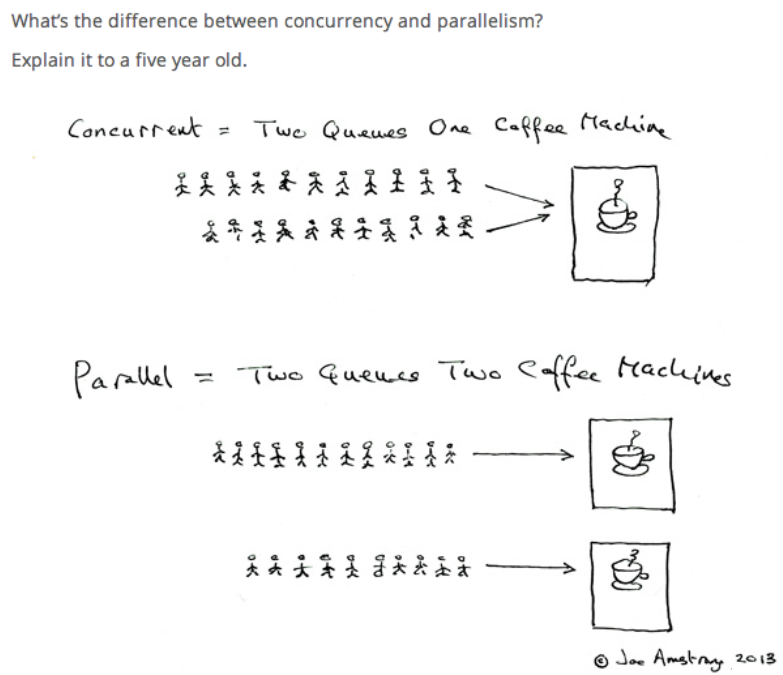
\includegraphics[width=0.75\textwidth]{images/EDP/concurrency_parallelism}
		\end{figure}
	\end{frame}
	
	\begin{frame}{Modelos de Concurrencia Basados en Eventos}
	Los modelos de concurrencia basados en eventos definen cómo las aplicaciones gestionan múltiples tareas simultáneamente mientras responden a eventos externos. Estos modelos garantizan un uso eficiente de los recursos y una capacidad de respuesta óptima. \newline
	
	\begin{itemize}
		\item \textbf{Single-Threaded vs. Multi-Threaded Event Processing}
		\item \textbf{Reactive \& Proactive Event Handling}
		\item \textbf{Callbacks, Promises, \& Async/Await}
		\item \textbf{Cooperative vs. Preemptive Concurrency}
	\end{itemize}	
	
	\end{frame}
	
	\begin{frame}{Modelos de Concurrencia Basados en Eventos}
		\justifying
	\textbf{Single-Threaded vs. Multi-Threaded Event Processing} \newline
	Las aplicaciones basadas en eventos pueden operar en entornos single-threaded o multi-threaded. En un modelo single-threaded, todas las tareas se ejecutan dentro de un único contexto de ejecución, a menudo utilizando un loop de eventos para gestionar operaciones asincrónicas. Este modelo es eficiente para tareas dependientes de E/S, pero puede convertirse en un cuello de botella para operaciones con un uso intensivo de la CPU. \\
	Por otro lado, un modelo multi-threaded permite la ejecución simultánea de múltiples tareas mediante el uso de subprocesos separados. Este enfoque mejora el rendimiento de las cargas de trabajo paralelizables, pero presenta desafíos como condiciones de carrera, deadlocks y sobrecarga de sincronización. La selección del modelo de subprocesos adecuado depende de los requisitos de concurrencia de la aplicación y de las características de la carga de trabajo.	
	\end{frame}

%	\begin{frame}{Single-Threaded vs. Multi-Threaded Event Processing}
%		\small
%	\begin{table}
%		\centering
%		\renewcommand{\arraystretch}{1.2}
%		\begin{tabular}{|p{3cm}|p{4cm}|p{4cm}|}
%			\hline
%			\textbf{Ventajas} & \textbf{Single-Threaded} & \textbf{Multi-Threaded} \\ \hline
%			 & Simplicidad &  Mejor utilizacón de la CPU \\ \hline
%			 & Evita Condiciones de Carrera & Ejecución más rápida para tareas que requieren un uso intensivo de la CPU \\ \hline
%			 & Eficiente para tareas de E/S &  \\ \hline
%			\textbf{Desventajas} & \textbf{Single-Threaded} & \textbf{Multi-Threaded} \\ \hline
%			& Utilización limitada de la CPU & Overhead de Sincronización \\ \hline
%			& Las operaciones de bloqueo retrasan la ejecución & Condiciones de Carrera y Deadlocks \\ \hline
%		\end{tabular}
%	\end{table}
%	\end{frame}
	
	\begin{frame}{Modelos de Concurrencia Basados en Eventos}
		
	\small
		\begin{columns}[T]
			\column{0.48\textwidth}
			
			\begin{block}{Single-Threaded}
				\textbf{Ventajas}
				\begin{itemize}
					\item Simplicidad
					\item Evita condiciones de carrera
					\item Eficiente para tareas de E/S
				\end{itemize}
				
				\vspace{0.2cm}
				\textbf{Desventajas}
				\begin{itemize}
					\item Utilización limitada de la CPU
					\item Bloqueos retrasan la ejecución
				\end{itemize}
			\end{block}
			
			\column{0.48\textwidth}
			
			\begin{block}{Multi-Threaded}
				\textbf{Ventajas}
				\begin{itemize}
					\item Mejor utilización de la CPU
					\item Mayor velocidad en tareas intensivas
				\end{itemize}
				
				\vspace{0.2cm}
				\textbf{Desventajas}
				\begin{itemize}
					\item Overhead de sincronización
					\item Condiciones de carrera y deadlocks
				\end{itemize}
			\end{block}
			
		\end{columns}
	\end{frame}
	

	\begin{frame}{Modelos de Concurrencia Basados en Eventos}
	\small
	\begin{table}
	\centering
	\renewcommand{\arraystretch}{1.2}
	\begin{tabular}{|p{3cm}|p{4cm}|p{4cm}|}
	\hline
	\cellcolor{blue!15}\textbf{Factor} & \cellcolor{blue!15}\textbf{Single-Threaded} & \cellcolor{blue!15}\textbf{Multi-Threaded} \\ \hline
	\cellcolor{blue!15}Mejor para & Tareas limitadas por E/S &  Tareas CPU-Intensivas \\ \hline
	\cellcolor{blue!15}Complejidad & Baja & Alta \\ \hline
	\cellcolor{blue!15}Perfomance & Eficiente con E/S asincrónicas & Alta para tareas en paralelo \\ \hline
	\cellcolor{blue!15}Sincronización & No necesaria & Requerida \\ \hline
	\end{tabular}
	\end{table}
	\end{frame}
	
	\begin{frame}{Modelos de Concurrencia Basados en Eventos}
	\textbf{Reactive \& Proactive Event Handling} \\
	\vspace{0.4cm}
	\justifying \small
	Las aplicaciones basadas en eventos pueden emplear estrategias de gestión \textbf{reactiva} o \textbf{proactiva}. La gestión \textbf{reactiva} de eventos implica responder a los eventos a medida que ocurren, sin anticipar interacciones futuras. Este enfoque es común en aplicaciones de interfaz de usuario (UI), servidores de red y sistemas en tiempo real, donde la aplicación espera la entrada y reacciona en consecuencia. \\ 
	Por el contrario, la gestión \textbf{proactiva} de eventos anticipa eventos futuros y prepara respuestas preventivas para optimizar el rendimiento. 
	Esta estrategia se utiliza en análisis predictivo, algoritmos de precarga y sistemas basados en IA.\\
	Ambos enfoques tienen sus ventajas: la gestión reactiva garantiza un uso mínimo de recursos, mientras que la gestión proactiva reduce la latencia de respuesta y mejora la experiencia del usuario.
	\end{frame}
	
	\begin{frame}{Modelos de Concurrencia Basados en Eventos}
		\small
		
		\begin{columns}[T]
			\column{0.48\textwidth}
			
			\begin{block}{Reactive Handling}
				\textbf{Ventajas}
				\begin{itemize}
					\item Eficiente en recursos
					\item Implementación más simple
					\item Escalable en Sistemas Asíncronos
				\end{itemize}
				
				\vspace{0.2cm}
				\textbf{Desventajas}
				\begin{itemize}
					\item Alta latencia
					\item Dependencia con Triggers externos
				\end{itemize}
			\end{block}
			
			\column{0.48\textwidth}
			
			\begin{block}{Proactive Handling}
				\textbf{Ventajas}
				\begin{itemize}
					\item Menor Tiempo de Respuesta
					\item Experiencia del Usuario Mejorada
					\item Utilización optimizada de recursos
				\end{itemize}
				
				\vspace{0.2cm}
				\textbf{Desventajas}
				\begin{itemize}
					\item Implementación compleja
					\item Procesamiento potencialmente innecesario
				\end{itemize}
			\end{block}
			
		\end{columns}
	\end{frame}
	
	\begin{frame}{Modelos de Concurrencia Basados en Eventos}
		\small
		\begin{table}
			\centering
			\renewcommand{\arraystretch}{1.2}
			\begin{tabular}{|p{3cm}|p{4cm}|p{4cm}|}
				\hline
				\cellcolor{blue!15}\textbf{Factor} & \cellcolor{blue!15}\textbf{Reactive Event Handling} & \cellcolor{blue!15}\textbf{Proactive Event Handling} \\ \hline
				\cellcolor{blue!15}Tiempo de respuesta & Alta latencia & Baja latencia \\ \hline
				\cellcolor{blue!15}Implementación & Simple & Compleja \\ \hline
				\cellcolor{blue!15}Mejor para & Interacciones UI, APIs & AI, prefetching, catching \\ \hline
				\cellcolor{blue!15}Uso de recursos & Eficiente & Puede ser innecesario \\ \hline
			\end{tabular}
		\end{table}
	\end{frame}
	
	\begin{frame}{Modelos de Concurrencia Basados en Eventos}
		
		\textbf{Callbacks, Promises, \& Async/Await} \\
		\vspace{0.4cm}
		\justifying \small
		La programación basada en eventos se basa en los métodos \textbf{Callbacks}, \textbf{Promises} y \textbf{Async/Await} para gestionar la concurrencia. Las \textbf{Callbacks} son funciones que se pasan como argumentos para gestionar eventos de forma asíncrona, comúnmente utilizadas en loops de eventos de JavaScript y Python. Sin embargo, el uso excesivo de \textbf{Callbacks} puede provocar un desastre, dificultando la gestión del código. \\
		Las \textbf{Promises} simplifican los flujos de trabajo asíncronos al representar un resultado futuro que puede tener éxito o fallar. Permiten el encadenamiento de operaciones, lo que reduce la complejidad. \\
		\textbf{Async/Await} mejora aún más la legibilidad al habilitar una sintaxis similar a la síncrona para el código asíncrono, lo que mejora la capacidad de mantenimiento y la depuración. \\
		Estos mecanismos constituyen la columna vertebral de los sistemas modernos basados en eventos, garantizando la ejecución fluida de operaciones no bloqueantes.
	\end{frame}
	
	\begin{frame}{Modelos de Concurrencia Basados en Eventos}
		\tiny 
		\begin{columns}[T]
			\column{0.30\textwidth}
			\begin{block}{Callbacks}
				\textbf{Ventajas}
				\begin{itemize}
					\item Simple y efectiva para tareas asincrónicas simples
					\item Funciona bien con listeners y handlers de eventos.
					\item Nativo para muchos lenguajes como JavaScript, Python y C.
				\end{itemize}
				
				\vspace{0.1cm}
				\textbf{Desventajas}
				\begin{itemize}
					\item Callback Hell
					\item Problemas de gestión de errores
				\end{itemize}
			\end{block}
			
			\column{0.30\textwidth}
			
			\begin{block}{Promises}
				\textbf{Ventajas}
				\begin{itemize}
					\item Mayor legibilidad que las Callbacks.
					\item Gestión de errores integrada con .catch().
					\item El encadenamiento permite flujos de trabajo asíncronos estructurados.
				\end{itemize}
				
				\vspace{0.1cm}
				\textbf{Desventajas}
				\begin{itemize}
					\item Aún requiere estructuras anidadas para tareas dependientes.
					\item Las promesas deben resolverse o rechazarse explícitamente.
				\end{itemize}
			\end{block}
			
			
			\column{0.30\textwidth}
			
			\begin{block}{Async/Await}
				\textbf{Ventajas}
				\begin{itemize}
					\item Elimina la anidación Callbacks y las cadenas de Promises.
					\item Legibilidad similar a la de un sistema síncrono con mejor gestión de errores.
					\item Ideal para tareas dependientes de E/S, como solicitudes de red y operaciones con archivos.
				\end{itemize}
				
				\vspace{0.1cm}
				\textbf{Desventajas}
				\begin{itemize}
					\item Requiere un loop de eventos (asyncio.run()).
					\item No es adecuado para tareas dependientes de la CPU sin Threads adicionales.
				\end{itemize}
			\end{block}
			
		\end{columns}
	\end{frame}
	
	\begin{frame}{Modelos de Concurrencia Basados en Eventos}
		\footnotesize 
		\begin{table}
			\centering
			\renewcommand{\arraystretch}{1.2}
			\begin{tabular}{|p{3cm}|p{2.5cm}|p{2.5cm}|p{2.5cm}|}
				\hline
				\cellcolor{blue!15}\textbf{Factor} &  \cellcolor{blue!15}\textbf{Callbacks} & \cellcolor{blue!15}\textbf{Promises}  & \cellcolor{blue!15}\textbf{Async/Await} \\ \hline
				\cellcolor{blue!15}Legibilidad & Baja & Moderada & Alta \\ \hline
				\cellcolor{blue!15}Manejo de errores & Complejo & Mejor & Simplificado \\ \hline
				\cellcolor{blue!15} Llamadas anidadas & Si & No & No \\ \hline
				\cellcolor{blue!15} Mejor Caso de Uso & Eventos simples & Tareas dependientes & Flujos de trabajo asincrónicos complejos \\ \hline
			\end{tabular}
		\end{table}
	\end{frame}
	
	\begin{frame}{Modelos de Concurrencia Basados en Eventos}
		
		\textbf{Cooperative vs. Preemptive Concurrency} \\
		\vspace{0.4cm}
		\justifying \small 
		La concurrencia en la programación basada en eventos puede ser \textbf{cooperativa} o \textbf{preventiva}. La concurrencia \textbf{cooperativa} se basa en que las tareas cedan el control voluntariamente para permitir la ejecución de otras tareas. Este enfoque es común en operaciones de E/S asíncronas, donde un loop de eventos determina el orden de ejecución. Minimiza la sobrecarga por cambio de contexto, pero puede provocar una inanición si las tareas no ceden.\\
		La concurrencia \textbf{preventiva}, en cambio, utiliza un scheduler externo para interrumpir forzosamente las tareas y asignar tiempo de CPU. Este modelo se utiliza ampliamente en aplicaciones y sistemas operativos multi-threaded, proporcionando equidad pero aumentando la complejidad de la sincronización. La elección entre estos modelos depende de los requisitos de concurrencia de la aplicación y las limitaciones de rendimiento. \\
		Los modelos de concurrencia basados en eventos determinan la eficiencia con la que las aplicaciones gestionan múltiples tareas. 
	\end{frame}
	
	
	\begin{frame}{Modelos de Concurrencia Basados en Eventos}
		\small
		
		\begin{columns}[T]
			\column{0.48\textwidth}
			
			\begin{block}{Cooperative Concurrency}
				\textbf{Ventajas}
				\begin{itemize}
					\item Bajo sobrecarga (Overhead)
					\item Ejecución predecible
					\item Eficiente para aplicaciones con E/S
				\end{itemize}
				
				\vspace{0.2cm}
				\textbf{Desventajas}
				\begin{itemize}
					\item Riesgo de bloqueo
					\item Requiere ceder manualmente
				\end{itemize}
			\end{block}
			
			\column{0.48\textwidth}
			
			\begin{block}{Preemptive Concurrency}
				\textbf{Ventajas}
				\begin{itemize}
					\item Mejor utilización de la CPU
					\item Previene la inanición
					\item Conmutación automática de tareas
				\end{itemize}
				
				\vspace{0.2cm}
				\textbf{Desventajas}
				\begin{itemize}
					\item Mayor sobrecarga
					\item Condiciones de carrera y bloqueos
					\item Depuración compleja
				\end{itemize}
			\end{block}
			
		\end{columns}
	\end{frame}
	
	\begin{frame}{Modelos de Concurrencia Basados en Eventos}
		\small
		\begin{table}
			\centering
			\renewcommand{\arraystretch}{1.2}
			\begin{tabular}{|p{3cm}|p{4cm}|p{4cm}|}
				\hline
				\cellcolor{blue!15}\textbf{Factor} & \cellcolor{blue!15}\textbf{Cooperative Concurrency} & \cellcolor{blue!15}\textbf{Preemptive Concurrency} \\ \hline
				\cellcolor{blue!15}Conmutación de Tarea & Voluntaria (await, yield) & Forzado por el SO \\ \hline
				\cellcolor{blue!15}Sobrecarga & Baja & Alta \\ \hline
				\cellcolor{blue!15}Ideal para & Tareas con restricciones de E/S  & Tareas con restricciones de CPU \\ \hline
				\cellcolor{blue!15}Factor de riesgo & Bloqueo por tareas largas & Condiciones de carrera, bloqueos \\ \hline
				\cellcolor{blue!15}Ejemplo de mecanismo & AsynIO, corrutinas & Threads, Multiprocesamiento \\ \hline
			\end{tabular}
		\end{table}
	\end{frame}
	
	\begin{frame}{Programación controlada por eventos}
		\Huge
		\centering
		¿Preguntas? 
		\begin{figure}[htb]
		\centering
		
\includegraphics[width=0.5\textwidth]{images/EDP/confused_emoji}
		\end{figure}
	\end{frame}	
	
	\begin{frame}{Programación controlada por eventos}
		\Huge
		\centering
		FIN 
		\begin{figure}[htb]
			\centering
			
\includegraphics[width=0.5\textwidth]{images/EDP/relaxed_emoji}
		\end{figure}
	\end{frame}	
%%	\section{Referencias}
%%	\begin{frame}[allowframebreaks]{Referencias}
%%		\bibliography{referencias}
%%	\end{frame}
%%	
%%	\begin{frame}
%%		
%%		\begin{center}
%%			Gracias!
%%			
%%			\email
%%		\end{center}
%%		
%%		\begin{figure}[htb]
%%			\centering
%%			\includegraphics[width=0.5\textwidth]{imagens/IB}
%%		\end{figure}
%%		
%%	\end{frame}
	
\end{document}